\documentclass{llncs}
\pagestyle{headings}
\usepackage{mathtools}
\usepackage{multirow, booktabs}
\usepackage{algorithm}
\usepackage[noend]{algpseudocode}
\usepackage{graphicx} 
\usepackage{amsmath}
\usepackage{amsfonts}
\usepackage{xcolor}
\usepackage{cases}
\usepackage{enumitem}


\DeclareMathSymbol{\shortminus}{\mathbin}{AMSa}{"39}
\newcommand{\var}{\mathit{var}}
\newcommand{\VAR}{\mathit{VAR}}
\newcommand{\Pos}{\mathit{Pos}}
\newcommand{\Neg}{\mathit{Neg}}
\newcommand{\trt}[1]{\texttt{#1}}
\newcommand{\mi}{\mathit}
\newcommand{\ve}{\mathbf}
\newcommand{\btablesize}{\begin{scriptsize}}
\newcommand{\etablesize}{\end{scriptsize}}
\newcommand{\set}[2]{\{{#1}\,|\,{#2}\}}
\newcommand{\lre}{\color{red}{\{}}

\newcounter{counterName}
\allowdisplaybreaks

%\makeatletter
%\renewcommand{\ALG@beginalgorithmic}{\footnotesize}
%\makeatother

\begin{document}

\title{A Decomposed Fourier-Motzkin Elimination Framework to Derive Capacity Models of Container Vessels}
\titlerunning{FME for Deriving Capacity Models}
\author{Mai L. Ajspur\inst{1} \and Rune M. Jensen\inst{1} \and and Kent H. Andersen\inst{2}}
\institute{The IT University of Copenhagen \and Aarhus University}

\maketitle

\begin{abstract}
Accurate Vessel Capacity Models (VCMs) expressing the trade-off between different container types that can be stowed on container vessels are required in core liner shipping functions such as uptake-, capacity-, and network management. Today, simple models based on volume, weight, and refrigerated container capacity are used for these tasks, which causes overestimations that hamper decision making.
Though previous work on stowage planning optimization in principle provide fine-grained linear Vessel Stowage Models (VSMs), these are too complex to be used in the mentioned functions. As an alternative, this paper contributes a novel framework based on Fourier-Motzkin elimination that automatically derives VCMs from VSMs by projecting unneeded variables. Our results show that the projected VCMs are reduced by an order of magnitude and can be solved 20-35 times faster than their corresponding VSMs with only a negligible loss in accuracy. 
% TODO: vist nok kun for dem med hydrostatik
Our framework is applicable to LP models in general, but are particularly effective on block-angular structured problems such as VSMs. We show similar results for a multi-commodity flow problem.
\keywords{Fourier-Motzkin Elimination \and Capacity Model \and Liner Shipping \and Projection.}
\end{abstract}

%\the\textfloatsep  22.76219pt plus 2.0pt minus 4.0pt
\setlength{\textfloatsep}{19.76pt plus 0.5pt minus 0.2pt}
%%%%%%%%%%%%%%%%%%%%%%%%%%%%%%%%%%%%%%%%%%%%%%%%%%%%%%%%%%%%%%%%%%%%%%%%%%%%%%%%%%%%%%%%%%%%%%%%
\section{Introduction}
Container shipping is a central element in the clockwork of global trade. %TODO: med vilje, du fjernede reference?
As part of this, container liner shipping companies operates a set of container vessels on services connecting major trade regions like Asia and Europe. Each company is focused on utilizing the cargo capacity in their service network, since unused capacity constitute a loss that can be fatal in a market with a profit margin of just a few percent. Thus, being able to estimate the residual capacity of a container vessel is central to the business. 
This is challenging in practice, however, since an empty slot may be impossible to utilize for a wide range of reasons, including the interaction of various stowage rules and seaworthiness requirements. As a result, the free capacity of each container type is a complex function of the composition of cargo on board the vessel and the design of the vessel. 

Usually, only the stowage planning team will be able to determine the residual capacity of a vessel accurately by spending hours of manual work. 
However, the knowledge is primarily needed in higher functions such as: {\em uptake management} that control the sale of cargo bookings to fill the vessels with profitable cargo; {\em capacity management} that route cargo through the service network; and {\em network management} that makes changes to the service network. Decision makers in these functions seldom have stowage insight or time to consult the stowage team. Instead, they usually boil down the free capacity of a vessel to its nominal volume, weight, and reefer (refrigerated containers) capacity minus total volume, weight and reefer number of containers already on board. This simple three dimensional capacity model is inherently optimistic, since it ignores stowage complications, and it has been shown that this can lead to revenue overestimates of more than 15\% \cite{AlbertosThesis}. This can cause sub-optimal decisions that significantly harm business. 
%
Previous work has contributed frameworks for automated stowage planning (e.g.,\cite{roach00,kimkang02,ambrosino04,pacino11}), and recently, linear stowage planning models were shown to scale to large container vessels (e.g., \cite{AlbertosThesis}). These latter Vessel Stowage Models (VSMs) embed an accurate capacity model, but since they include positioning information about the containers, they are too large for use as capacity models in higher functions, since these tasks often require several hundred capacity models to be solved simultaneously.

In this paper, we introduce a novel method to calculate a Vessel Capacity Model (VCM) automatically from a VSM. Our basic idea is to derive the VCM by projecting out positioning variables from the VSM, such that the VCM only expresses the relationship between variables representing the total amount of each possible container type. Despite a theoretical double-exponential complexity, Fourier-Motzkin Elimination (FME) has been applied successfully in previous work in domains including constraint programming (e.g., \cite{lassez90}) and software verification (e.g., \cite{benoy05}). Our main contribution is to improve the state-of-the-art of these FME-based projection frameworks (e.g., \cite{simon05,lukatskii08,shapot12}). In particular, we introduce a novel decomposition method that takes advantage of block-angular structured models such as VSMs to significantly speed-up the projection of variables in these models. Additionally, our removal of redundant constraints is parallellized, and the framework includes preprocessing of the constraint system including removal of less strict inequalities.

Our experimental evaluation of computing VCMs with this method shows that the number of constraints and non-zeros in the resulting VCMs typically are reduced by an order of magnitude compared to their corresponding VSMs. The decomposition reduces the size of the intermediary systems produced by FME, causing less time to be needed for removing redundant constraints, which speeds up the projection process significantly. In addition, for the models that include hydrostatic constraints, the resulting VCMs can be solved 20-35 times faster than their VSMs with only a negligible loss in accuracy. Although it can take several hours to derive a capacity model due to the clean-up of redundant constraints, this only has to be done one time for a vessel class, making the approach suitable for computing these models. Since the VCMs are linear and much faster to solve than their corresponding VSMs, they can be integrated in decision support systems for the higher functions in liner shipping. Multi-commodity flow problems also have a block-angular structure and we found a speed-up and a reduction in final size similar to the ones seen for VCMs.

This paper is organized as follows. Section~\ref{sec:notation} introduces the required definitions and notation, % for our FME framework, 
and Section~\ref{sec:model} briefly presents the VSMs that are projected. Then Section~\ref{sec:method} outlines the methods used in our FME framework including how block-angular problems are decomposed. Our experimental results then follows in Section~\ref{sec:results}. Section~\ref{sec:relatedwork} presents related work, before Section~\ref{sec:conclusion} concludes.
%%%%%%%%%%%%%%%%%%%%%%%%%%%%%%%%%%%%%%%%%%%%%%%%%%%%%%%%%%%%%%%%%%%%%%%%%%%%%%%%%%%%%%%%%%%%%%%%%%%%%%%%%%%%%
\section{Definitions and notation} \label{sec:notation}
A constraint system $S$ is a set of linear equalities and inequalities over the same set of continuous variables, $\VAR(S)=\{x_1,\ldots, x_n\}$.  
For the constraint $c\in S$, we let $\var(c)$ denote the variables whose coefficient in $c$ is nonzero and say that $c$ \emph{uses} $x$ if $x\in \var(c)$. 
The set of points in $\mathbb{R}^n$ that satisfies all constraints in $S$ is called the \emph{feasible area} of $S$. A constraint $c\in S$ is \emph{redundant} iff removing it from $S$ does not influence the feasible area of $S$, otherwise it is called \emph{non-redundant}.  

For some variables $Y\subseteq \VAR(S)$, we are not interested in their values in a feasible point - we just want to know that a satisfying value exists. This is captured by the \emph{projection of $S$ w.r.t. $Y$}, which is the largest set consisting of values for $\VAR(S)\setminus Y$ that can be extended with values for $Y$ such that all constraints in $S$ are satisfied. 
%
The projection of a constraint system is a uniquely determined subset of $\mathbb{R}^{n-|Y|}$, but also the feasible region of another system $S'$ (see e.g. \cite{ziegler95}). We are mostly interested in the latter, since it is the relationship between the values in the projection that is relevant to us, and we will allow ourselves to write that ``$S'$ is the projection of $S$ w.r.t. $Y$'' if the feasible area of $S'$ equals the projection of $S$, though such a system is not uniquely determined.
We note, that since we are dealing with subsets of multi-dimensional Euclidian spaces, the dimension and the order of the variables are important. However, in order to simplify the presentation, we do not explicitly specify these for every considered projection/constraint system $S'$. A more stringent exposition keeping track of the variable sets and ordering can be found in \cite{mytechrep}.

%%%%%%%%%%%%%%%%%%%%%%%%%%%%%%%%%%%%%%%%%%%%%%%%%%%%%%%%%%%%%%%%%%%%%%%%%%%%%%%%%%%%%%%%%%%%%%%%
\section{Vessel Stowage Model}\label{sec:model}
A Vessel Stowage Model (VSM) is a constraint system defining the feasible stowage conditions of a vessel. For a stowage condition to be feasible, the vessel must among other things be seaworthy with proper transversal stability and stress forces within given limits (hydrostatic constraints); capacities should not be exceeded; the container stacks must by physically possible (e.g., 20' containers cannot be stowed on top of 40' containers); and there are separation rules for dangerous cargo to name a few. For an in-depth coverage of container vessel stowage, the reader is referred to a recent book on the topic \cite{JPAV18}.     

Consider the container vessel shown in Figure~\ref{fig:vessel}. Each \emph{cell} on the vessel can hold two 20' containers or one 40', and some cells have power plugs, allowing refrigerated containers (\emph{reefers}) to be stowed. Container stacks are arranged longitudinal in \emph{bays} that can be further subdivided into \emph{locations}, and each stack rests on sockets with maximum weight limits. To help achieve stability of the vessel, large water ballast tanks are placed on the vessel.
The volume capacity of a vessel is measured in Twenty-foot Equivalent Units (TEUs) and can be more than 20K. 

\begin{figure}[tb]
	\centering
		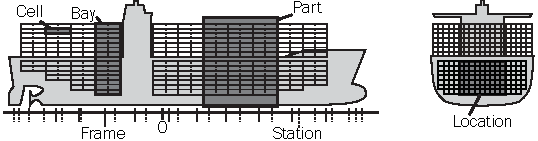
\includegraphics[scale = 0.9]{figures/vessel6.pdf}
	\caption{Vessel structure and reference points.}
	\label{fig:vessel}
\end{figure}

The VSMs used in this paper is based on previous work on stowage planning optimization (e.g., \cite{pacino11,AlbertosThesis}).  
They considers 20' and 40' containers in three weight classes, and a container is either reefer or non-reefer. This gives a total of 12 container types $T$. 
For each container type and location on the vessel, a decision variable defines the number of containers of the type in the location. Due to the large number of containers, we ignore the integrality of these variables as in \cite{pacino11}. 
The models are based on industrial data from a large carrier and include a number of volume, weight and reefer capacity constraints for each location. The data specifies hydrostatic limits at \emph{frame positions}, while input for hydrostatic calculations are given at other \emph{station positions} (see Figure~\ref{fig:vessel}). A simplification of the representation of the hydrostatics is achieved by dividing the vessel into \emph{parts} ($P$) spanning one or more succeeding bays or no bays at all as shown in Figure~\ref{fig:vessel}. 
The weight of ballast water in each part is given by a continuous decision variable, and hydrostatic constraints are included that restrict the shear forces and bending moments at positions between parts. To this end, the model includes constraints defining the resulting force on each part using a linear approximation of its buoyancy and weight. The hydrostatic modeling approach of the VSM and the quality of the approximations are detailed in \cite{ICCL18}. 
%
A Vessel Capacity Model (VCM) is derived from a VSM by adding auxiliary variables that equals the total of each container type on board the vessel and projecting all other variables out using FME. In this way the container positioning information is abstracted away.

Due to space limitations, we do not include a formal definition of the VSMs on which our experiments are carried out. However, it can be found in \cite{mytechrep}. 
Instead, to explain our FME framework we briefly introduce the toy version VSM below. For this VSM, merely the structure is essential while the constraints themselves are of less importance.
\begin{small}
\begin{numcases}{S_p\text{ for all parts }p\in P:} 
	\smashoperator[lr]{\sum_{\tau \in T^\trt{20}}} x_{p,\tau} \leq C_p^\trt{20}                         
			& $\smashoperator[lr]{\sum_{\tau \in T^\trt{40}}} 2 x_{p,\tau} \leq C_p^\trt{40}$ \label{eq:capVol}\\
 \smashoperator[lr]{\sum_{\tau \in T^\trt{20}}} W_\tau x_{p,\tau} \leq C_p^\trt{W20} 
	    & $\smashoperator[lr]{\sum_{\tau \in T^\trt{20}}}0.5 W_\tau x_{p,\tau} + \smashoperator[lr]{\sum_{\tau \in T^\trt{40}}} W_\tau  x_{p,\tau} \leq C_p^\trt{W40}\quad$ \label{eq:capW}\\ 
	\smashoperator[r]{\sum_{\tau \in T^\trt{R}}} x_{p,\tau} \leq C_p^\trt{R}
      & $\smashoperator[lr]{\sum_{\tau \in T^\trt{20}}} x_{p,\tau} + \smashoperator[lr]{\sum_{\tau \in T^\trt{40}}} 2x_{p,\tau} \leq C_p^\trt{TEU}$ \label{eq:capReefer}
\end{numcases}
\begin{numcases}{S_\texttt{g}:}
	x_\tau = \sum_{p\in P} x_{p,\tau} & $\forall{\tau \in T}$\label{eq:sumT}\\
	\sum_{p\in P}\sum_{\tau\in T}W_\tau x_{p,\tau} \leq D\label{eq:sumW}
\end{numcases}
\end{small}
In this model, the only decision variables are the $x_{p,\tau} \in \mathbb{R}$, which denotes the number of containers in part $p\in P$ of type $\tau$. \eqref{eq:capVol} defines the volume capacity of part $p$ of 20' and 40' containers, while \eqref{eq:capW} defines the weight capacity of 20' and 40' containers, respectively ($W_\tau$ is the weight of type $\tau$). We notice that the weight limits of 40' containers includes half of the weight of 20' containers due to the arrangement of sockets, and that a 40' container counts two TEU. \eqref{eq:capReefer} defines reefer and total TEU capacity of part $p$, respectively. 
Constraint \eqref{eq:sumT} defines the auxiliary variables $x_\tau$ that totals the container types (i.e., the only variables that will be left in the VCM), while \eqref{eq:sumW} limits the total weight of cargo.

This presentation clearly exposes the VSMs natural (primal) block-angular structure \cite{williams}: For each part $p$, $S_p$ is a set of capacity constraints for part $p$ that constitutes a local system, whose constraints only use variables that are not used in $S_{q}$ for a different part $q$. The remaining constraints make up the global subsystem, $S_\texttt{g}$, where the constraints also use variables from several of the local subsystems.
%%%%%%%%%%%%%%%%%%%%%%%%%%%%%%%%%%%%%%%%%%%%%%%%%%%%%%%%%%%%%%%%%%%%%%%%%%%%%%%%%%%%%%%%%%%%%%%%%%%%%%
\section{FME-based projection framework} \label{sec:method}
Our projection framework based on Fourier-Motzkin Elimination (FME) can be used for massive variable elimination in any linear inequality system but has been designed to take advantage of the block-angular structure often found in real-world models including the VSMs. The methods for projecting a constraint system are described in Section~\ref{sec:projMethod}, while the decomposition used on block-angular structured problems is described in Section~\ref{sec:decomp}.

\subsection{Projection procedure}\label{sec:projMethod}
The projection procedure starts with a preprocessing of the constraint system $S$.
Then we use the equalities in the reduced system to isolate variables from $Y$ and substitute in the rest of the system (Gauss-eliminations).  
Subsequently, we successively eliminate one variable from $Y$ at a time using FME and remove redundant inequalities. At the top-level, the pseudocode for our projection method is therefore as described in Algorithm~\ref{alg:FMEF}. Each sub-procedure in this algorithm is detailed below. 

\setlength{\floatsep}{10pt} %standard minimum er vist 16
\setlength{\textfloatsep}{14pt} %standard minimum er vist 16
\begin{algorithm}[b!]
\caption{Projection based on Fourier-Motzkin elimination} 
\label{alg:FMEF}
\begin{algorithmic}
\Function{Project}{System $S$, Variables $Y$}
	\State $(S,Y)\gets \Call{Preprocess}{S,Y}$
	\State $(S,Y)\gets\Call{Gauss-Elim}{S,Y}$
	\While{$Y\neq\emptyset$}
		\State $(S, Y, New )\gets\Call{FME-SingleVar}{S,Y}$
		\State $S\gets\Call{RemoveRedundancy}{S,New}$
	\EndWhile
	\State \Return $S$
\EndFunction
\end{algorithmic}
\end{algorithm}

{{\sc Preprocess}$(S,Y)$:} We reduce $S$ by removing easily identifiable redundant constraints and assign necessary bounds and values to variables using well-known LP preprocessing steps (e.g., \cite{andersen95}). %TODO and more
We further perform FME on variables in $x\in Y$ in easy cases where this only results in a deletion of a set of inequalities or a substitution of a variable with a value (when $|\Pos_S(x)|$ or $\Neg_S(x)|$ is 0 or 1, see further below). We remove a redundant inequality when it is \emph{linearly dependent} or \emph{less strict} than another. This can be seen syntactically and happens in some of the cases when two constraint $c$ and $c'$ have the same coefficients (modulo a constant), or the coefficient in $c$ is dominated by the coefficients in $c'$ (modulo a constant). 
The steps are implemented with special care of equalities and working with the assumption that the system is feasible (details can be found in \cite{mytechrep}).

{{\sc Gauss-Elim}$(S,Y)$:} An equality $e$ can be used to isolate a variable $x\in Y$ which can then be substituted in all other constraints in $S$ (a Gauss-elimination). This eliminates $x$ from the system and does not cause the same combinatorial explosion of inequalities as FME may do (e.g., \cite{duffin74,simon05}).
To avoid density, when the system $S$ contains several equalities, we choose the variable $x$ (used in any equality) that is used the fewest times in total in $S$ and the equation $e$ (among those using $x$) that uses the fewest variables. 
This is repeated until there are no more equalities using variables in $Y$.

{{\sc FME-SingleVar}$(S,Y)$:} FME is a classical algorithm for producing the projection of a set of variables from a system where all constraint are inequalities on the form $\ve{a}\cdot \ve{x}\leq b$. The method successively eliminates one variable $x\in Y$ until all required variables have been eliminated. To eliminate $x\in Y$, the constraints in $S$ are first divided into three sets, $\Pos_S(x)$, $\Neg_S(x)$, and $\mi{Zero}_S(x)$ depending on the sign of the coefficient of $x$. Here, bounds are treated as any other inequalities. 
A new system $S'$ is then created, which is the projection of $S$ w.r.t. $\{x\}$. It consists of $\mi{Zero}_S(x)$, together with one inequality, $i_{p,n,x}$, for each pair $(p,n)\in \Pos_S(x)\times \Neg_S(x)$. $i_{p,n,x}$ is the addition of positive multiples of $p:\ve{a}\cdot\ve{x} \leq b$ and $n:\ve{a}'\cdot\ve{x} \leq b'$ such that the coefficient of $x$ in the resulting inequality is $0$. That is, $i_{p,n,x}$ equals $-a'_x\cdot \ve{a}\cdot\ve{x} + a_x\cdot \ve{a}'\cdot\ve{x} \leq -a'_x\cdot b + a_x\cdot b'$, where $a_x$ and $a'_x$ is the coefficient of $x$ in $c$ and $c'$, respectively,

The order in which variables are eliminated naturally influences the size of the intermediary constraint systems. We have chosen to use the greedy heuristic {that minimizes the number of new inequalities in the immediately next system \cite{duffin74}}, which is a commonly used heuristic and easily calculated from the current system. % as the variable $x\in Y$ that minimizes $|\Pos_S(x)||\Neg_S(x)| - |\Pos_S(x)|-|\Neg_S(x)|$.  
In the worst case scenario, %where $|\Pos_S(x)| = |\Neg_S(x)| = \frac{|S|}{2}$ for all $x\in Y$, 
the number of inequalities in the created system $S'$ is $\frac{1}{4}|S|^2$, which implies that (both time and space) complexity is double-exponential. For a large, dense system, the growth will be substantial, which prohibits it from use for practical purposes \emph{if} the added inequalities are non-redundant or the non-redundant inequalities are not removed ({see e.g. \cite{lukatskii08}}). It should, however, also be emphasized that not all inequalities in the succeeding system are necessarily non-redundant; in fact, the number of non-redundant inequalities will at most grow exponentially \cite{monniaux10}.

{{\sc RemoveRedundancy}$(S,\mathit{New})$:} To detect redundancy, we examine each inequality $c: \ve{a}\cdot \ve{x}\leq b$ in turn and remove it from the system if $\max \ve{a}\cdot \ve{x}$ subject to $S\setminus\{c\}$ is less than or equal to $b$. The property can be checked using an LP solver. Equalities are not examined, since we want to keep these for use in Gauss-elimination. When removing redundancy after projecting $x$ from $S$, we only check the newly added inequalities; if a constraint in $\mi{Zero}_S(x)$ is non-redundant before the elimination, it will be non-redundant afterward as well. 
%
For large systems, checking all constraints for redundancy is time-consuming. We have therefore implemented a method for redundancy removal that uses several threads in parallel. Each thread checks one inequality at a time, while a manager takes care of the communication and keeps track of the redundant inequalities. 

Several of the constants in the data used for our VSMs are results of various approximations and hence the boundary of the feasible area is not exact. Coarsening the boundary is therefore permissible, and we also remove inequalities that are \emph{``almost redundant''}. An inequality $c: \ve{a}\cdot\ve{x}\leq b$ is almost redundant if $\max \ve{a}\cdot\ve{x}$ subject to $S\setminus\{c\}$ is less or equal to $b + \epsilon\cdot |b|$ for a small $\epsilon$. 
Therefore, the manager also collects a set of almost redundant inequalities. After the parallel redundancy check, \emph{one} thread is then used to go through all the almost redundant inequalities sequentially, and the ones that are still almost redundant are removed. 
%Methods for coarsening the boundary of the feasible area are also used in \cite{lukatskii08,shapot12}.
%%%%%%%%%%%%%%%%%%%%%%%%%%%%%%%%%%%%%%%%%%%%%%%%%%%%%%%%%%%%%%%%%%%%%%%%
\subsection{Decomposing a block-angular system}\label{sec:decomp}
The toy VSM from Section~\ref{sec:model} has a natural block-angular structure, where the set of capacity constraints for each part constitute a local subsystem ($S_p$ for $p\in P$), and the remaining constraints form a global subsystem ($S_\texttt{g}$). 
To derive the VCM from this VSM, we want to eliminate all variables except those counting the number of containers of each type. However, when a variable $x_{p,\tau}$ is eliminated, the new inequalities constructed by FME uses variables from all subsystems, since $x_{p,\tau}$ is used in the global constraints that are combined with constraints from $S_p$. Continuing with FME, this result in an increasing number of global and more dense constraints, which again makes FME perform worse. 
To avoid the immediate ``mix'' of local subsystems, we will define and use auxiliary variables to ensure that we can project the local subsystems separately without producing global constraints. Afterward, we combine the projected subsystems and eliminate the auxiliary variables. 

For the considered toy VSM, we first define a variable to hold the weight of cargo in each part $p$, $w_p$. We also define the variables $x'_{p,\tau} = x_{p,\tau}$, though this merely appears to be a renaming of variables. For each $p$, we then add the definition of $w_p$ and $x'_{p,\tau}$ to $S_p$ and rewrite the global constraints in terms of the new variables. 
That is, local subsystem $p$ is now $S_p^0 = S_p \cup \{w_p = \sum_{\tau\in T} W_\tau x_{p,\tau}\} \cup \bigcup_{\tau\in T}\{x'_{p,\tau} = x_{p,\tau}\}$, while the new system of global constraints is $S_\texttt{g}^0 = \cup_{\tau\in T}\{x_\tau = \sum_{p\in P} x'_{p,\tau}\} \cup \{\sum_{p\in P} w_p \leq D\}$. 
%
Notice that due to the new variables, none of the variables $x_{p,\tau}$ for a given $p$ is used in any constraints outside of $S^0_p$. Therefore, to project $\set{x_{p,\tau}}{\tau\in T}$ for a given $p$ from the whole system ($S^0_\texttt{g}\cup\bigcup_{q\in P}S^0_{q}$) we can start by just eliminating $\set{x_{p,\tau}}{\tau\in T}$ from $S_p^0$. Then we can do so for the other parts. When all subsystems $S^0_p$ have been projected, we can join these projections together with $S^0_\trt{g}$ and eliminate the remaining variables, $\set{x'_{p,\tau}}{\tau\in T, p\in P}\cup\set{w_p}{p\in P}$, from the resulting system.

More formally, for a block-angular structured system with local subsystems $S_1,\ldots, S_k$ (using the variables $X_1,\ldots, X_k$) and global subsystem $S_\texttt{g}$
we do as follows for all subsystems $S_i$ (detailed pseudocode and correctness proofs can be found in \cite{mytechrep}). 
\begin{itemize}[noitemsep,topsep=0pt]%\itemsep0em
\item For each global constraint $c$ using variables in $S_i$, we define an auxiliary variable $z^0_{c,i}$ that equals the variables in $S_i$'s contribution to $c$. We add the equality defining $z^0_{c,i}$ to $S_i$, and we substitute it in $c$. 
We name the produced subsystem $S_i^0$. 
\item Then, we project $S_i^0$ w.r.t. all variables from $Y\cap X_i$, resulting in the system $S'^{\,0}_i$. We \emph{do keep} the auxiliary $z^0$-variables. 
\end{itemize}
After projecting each $S_i^0$ we combine the projections with $S_\trt{g}^0$ to create $\mathcal{S} \overset{\text{def.}}{=}S^0_\trt{g} \cup S'^{\,0}_1\cup \ldots \cup S'^{\,0}_k$.
We then eliminate from $\mathcal{S}$ all the auxiliary $z^0$-variables, $Z^0$, plus any remaining variables in $Y$. 

Comparing $\mathfrak{S} \overset{\text{def.}}{=} S_1^0\cup\ldots\cup S_k^0\cup S_\trt{g}^0$ with the original system $S$, all we have done is defining auxiliary variables and substituted them in the system. Thus, eliminating $Y$ from $S$ is equivalent to eliminating $Y \cup Z^0$ from $\mathfrak{S}$. 
%
When eliminating $Y\cup Z^0$ from $\mathfrak{S}$, we can choose to first eliminate $X_1\cap Y$, then $X_2\cap Y$ up to $X_k\cap Y$, and finally $Z^0\cup Y\setminus(X_1\cup \ldots\cup X_k)$. 
Any variable in $X_1\cap Y$ has a zero-coefficient in all constraints outside $S^0_1$, so $\mathfrak{S}\setminus S^0_1$ will not be changed by FME when $X_1\cap Y$ is eliminated. It can therefore be put aside until that projection is done. 
Likewise, when eliminating $X_i\cap Y$, neither $S_{i+1}^0\cup \ldots \cup S_k^0\cup S_\trt{g}^0$ nor the already projected systems contain any variables from $X_i\cap Y$ and can hence be put aside until the variables in $Z^0\cup Y\setminus(X_1\cup \ldots\cup X_k)$ are eliminated. Thus, the following holds. 
%
\begin{proposition}
The projection of $S$ w.r.t. $Y$ defines the same feasible area as 
the projection of $\mathcal{S}$ w.r.t. $Z^0 \cup Y\setminus (X_1\cup \ldots \cup X_k)$. 
\end{proposition}
%
$\mathcal{S}$ has by construction a block-angular structure and instead of eliminating the remaining variables immediately, we can use the same approach as above to postpone ``mixing'' blocks if for example the global constraints use too many variables. 
As an example, consider again the toy VSM that was decomposed into the subsystems $S^0_\trt{g}$ and $S^0_p$ for $p\in P$ and assume that $P=\{1,2,3,4\}$. Then we can group the subsystems into two groups, $\{S^0_1, S^0_2\}$ and $\{S^0_3, S^0_4\}$, and for each global constraint define a variable stating each new group's contribution to the global constraint. For example, for the global constraint $w_1 + w_2 + w_3 + w_4 \leq D$, we define a variable $w_{\{1,2\}}$ that is the weight of the containers in part 1 and 2. We similarly define $w_{\{3,4\}}$ and substitute with these in the global constraint. In total, we construct the following subsystems that can be arranged in a tree structure as shown in Figure~\ref{fig:decomp2}(a).
\begin{footnotesize}
\begin{align*}
S_\trt{g}^1 &:\cup_{\tau\in T}\{ x_\tau = x'_{\{1,2\},\tau} + x'_{\{3,4\},\tau}\} \cup \{ w_{\{1,2\}} + w_{\{3,4\}} \leq D \},\\   
S^1_1				&:\cup_{\tau\in T}\{ x'_{\{1,2\},\tau} = x'_{1,\tau} + x'_{2,\tau}\}\cup \{ w_{\{1,2\}} = w_{1} + w_{2}\},\\
S^1_2				&:\cup_{\tau\in T}\{ x'_{\{3,4\},\tau} = x'_{3,\tau} + x'_{4,\tau}\} \cup \{ w_{\{3,4\}} = w_{3} + w_{4}\}. 
\end{align*}
\end{footnotesize}
To obtain the projection of the original toy VSM, these systems are then projected recursively as shown in Figure~\ref{fig:decomp2}(b).
%
\begin{figure}[bt]
	\centering
		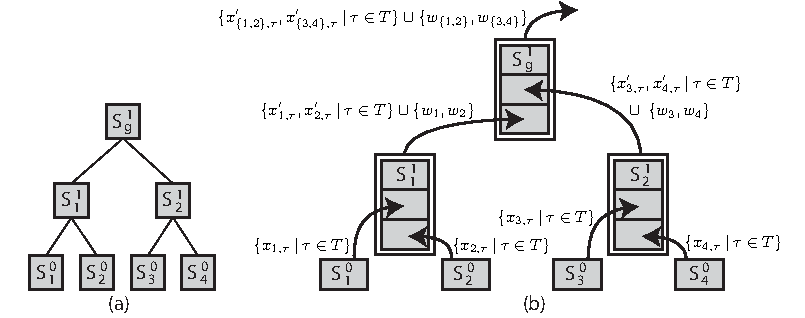
\includegraphics[scale=0.9]{figures/Example6.pdf}
	\caption{(a) Tree-strucure of subsystems. (b) Projection using tree-structure from (a).}
	\label{fig:decomp2}
\end{figure}

In more general terms, we divide all subsystems into $k$ groups and do the following for $1\leq j\leq k$. 
\begin{itemize}[noitemsep,topsep=0pt]%\itemsep0em
\item We define a system $S^1_j$. For each global constraint $c$ using variables from systems in group $j$, we define a variable, $z^1_{c,j}$, that equals the contribution to $c$ made by the variables in the systems in group $j$. We add the defining equality to $S^1_j$ and rephrase $c$ using $z^1_{c,j}$.
\item Then we project $S^1_j$, w.r.t. the previous, auxiliary $z^0$-variables, while we do keep the newly created $z^1$-variables.
\end{itemize} 
Subsequently we can then join the projected $S^1$-systems with the new global constraints, and finally project the last auxiliary variables. Alternatively, we can repeat the steps above until the final projection can be done. 

When we decompose a system as described above, we effectively create a tree structure of subsystems paired with a set of variables to be eliminated. An inequality system can then be projected by recursively projecting its children as shown in Figure~\ref{fig:decomp2}.
The intuition why this works is as before; projecting all $Y$ and $Z$-variables from the union of all the (unprojected) subsystems in the tree corresponds to projecting the $Y$ variables from $S$, and because we can choose the elimination order of the variables, we only need to project the subsystems in the tree in the correct order (a rigorous proof can be found in \cite{mytechrep}).

\begin{proposition}
The projection of the system associated with the root of the tree constructed from $S$ and $Y$ w.r.t. the $Y$- and $Z$-variables as described corresponds to projecting $S$ w.r.t. $Y$.
\end{proposition}

Using our previously described projection method, we obtain the projection of $S$ w.r.t. $Y$ by calling \Call{ProjectNode}{root of $T$}, where $T$ is the tree structure constructed from $S$ and $Y$, and \Call{ProjectNode}{} is described in Algorithm~\ref{alg:decomp}. We note that due to the elimination of almost redundant inequalities, this only
approximates the projection. However, by setting $\epsilon = 0$, the algorithm indeed returns the correct projection.
\begin{algorithm}[tb]
\caption{{Projecting a block-structured system via decomposition.}}
\label{alg:decomp}
\begin{algorithmic}
\Function{ProjectNode}{Node $n$} 
	\State $(S,Y)\gets$ the system and variable set associated with $n$
	\If{$n$ is a leaf}
		\State \Return \Call{Project}{$S$, $Y$}\Comment Algorithm~\ref{alg:FMEF}
	\Else
		\ForAll{children $m$ of $n$}
			\State $S \gets S\cup \Call{ProjectNode}{m}$ 
		\EndFor
		\State \Return $\Call{Project}{S, Y}$ \Comment Algorithm~\ref{alg:FMEF}
	\EndIf
\EndFunction
\end{algorithmic}
\end{algorithm}

Using the described decomposition, it is of course also possible to project nested block structured problems, i.e. systems that on the top-level can be divided into a global part and a number of local parts that in themselves can be further divided into local parts and a global part, and so on. Other block structured problems such as staircase problems can also be decomposed into a tree structure and projected using the described approach. 
%
Further, when the system $S$ is decomposed into subsystems in a tree structure, the projection itself can be parallelized by maintaining a queue of not yet projected subsystems whose children have all been projected. The members of the queue (which initially are the leafs) are then projected independently in parallel. %, which means that the total number of threads must be [kept in check/monitored/controlled.

%%%%%%%%%%%%%%%%%%%%%%%%%%%%%%%%%%%%%%%%%%%%%%%%%%%%%%%%%%%%%%%%%%%%%%%%%%%%%%%%%%%%%%%%%%%%%%%%%%%%%%%%%%%%%%
\section{Results}\label{sec:results}
We have constructed a number of different VSMs for a specific vessel, where the weight and hydrostatics are taken into account to various degrees. The first VSM %has no limit on the total displacement or any hydrostatic constraints, the second VSM 
does not model any hydrostatic constraints (similar to the toy-example but with more capacity constraints), and the subsequent VSMs (refered to as complex VSMs) consider stress force  constraints at the endpoint of 2, 4, 6 and 8 sections, respectively. 
Each VSM has been transformed into its corresponding VCM by eliminating all variables except the $x_\tau$ variables. Projections have been done in two different ways, \emph{decomposed} and \emph{flat}. For the decomposed projections, a tree structure has been used as described in Section~\ref{sec:decomp}, while the flat projections do not use any decomposition at all. CPU time is measured in both number of iterations and \emph{ticks} calculated by the CPLEX Interactive Optimizer version 12.5.0.0. Our FME-based projection framework has been implemented in Java. The experiments were carried out on a computer with an {Intel\textsuperscript{\textregistered} Xeon\textsuperscript{\textregistered} CPU with 8 cores and 32GB RAM.}

Table~\ref{tab:projections} shows the size reductions of the VCMs. It summarizes the size of the VSMs and the VCMs that are the result of the projection using decomposition. These sizes are given in terms of the number of inequalities (ineq), equalities (eq), variables (var), non-zero entries (nzs) and density (dens). The size of the VSMs are given both as they appear as input to our algorithm, and after it has been preprocessed by CPLEX. For comparison, the table includes a "Simple VCM" corresponding to the maximum volume, weight, and reefer capacity models used in liner shipping today.   
\begin{table}[tb]
\caption{The size of the VSMs and corresponding VCMs.}
\label{tab:projections}
\centering
\btablesize
\begin{tabular}{l|*{2}{*{3}{r@{\:\;}}r|}*{3}{r@{\:\;}}r}
$\multirow{2}{*}{}$&\multicolumn{4}{c|}{VSM}&\multicolumn{4}{c|}{VSM, presolved}& \multicolumn{4}{c}{VCM}\\
							&ineq (eq)&var &nzs & dens  &ineq &var	&nzs	&dens&ineq &var &nzs &dens\\
\hline
%{No weights}	&774 (12)	&1142&6662&8.61		&554	&657	&2784	&5.03&	20 &12	& 155&7.75\\   %554/20 = 27,7, 657/12 = 54,74,  2785/155 = 17,97
{No hydro.} 	&806 (43)	&1173&7854&9.74		&555	&657	&3441	&6.20&	18 &12	& 144&8.00 \\  %555/18 = 20,8, same							3441/144 = 23,89
{2 sections}	&810 (43)	&1173&7860&9.70		&556	&661	&3447	&6.20&	96 &12	&1113&11.59\\  %556/96 = 5,8, 661/12 = 55				3447/1113 = 3,09
{4 sections}	&824 (49)	&1179&7886&9.57		&564	&671	&3471	&6.15&	64 &12	& 731&11.42\\  %564/64 = 8,8										3471/731 = 4,74
{6 sections}	&838 (55)	&1185&7916&9.44		&570	&679	&3496	&6.13&	80 &12	& 888&11.10\\  %570/80 = 7,1										3496/888 = 3,94
{8 sections}	&852 (61)	&1191&7950&9.33		&576	&685	&3522	&6.11&	52 &12	& 582&11.19\\  %576/52 = 11,1 685/12 = 57.1			3522/582 = 6,05
\bottomrule
Simple VCM 		& 3\phantom{ (55)}&12 &\phantom{12}36&12.00&3&9&\phantom{12}24&\multicolumn{1}{l}{8.00}\\
\end{tabular}
\etablesize
\end{table}
Since we project all but 12 variables, this naturally gives a large reduction in the number of variables (54-57 times fewer than the presolved VSMs). However, the VCMs also have 5.8-11.8 times fewer inequalities than the presolved VSMs for complex VSMs % while they two others have 20.8-27.7 times fewer constraints. 
(20.8 for the first model).
The VCMs also have fewer non-zero entries (3-6 times fewer for complex VSMs, otherwise 24). The results reveal no apparent relationship between the size of the VSM and the size of its VCM.

Regarding the decomposition impact, Table~\ref{tab:time} shows the time taken for the algorithm to do the projection, both decomposed and flat. For most VSMs, the flat projection timed out (TO) beyond 18 hours, in which case the variables left to be projected are given. Figure~\ref{fig:8parts}(a) shows the progression of the number of inequalities and variables, respectively, as a function of time when the algorithm runs on the decomposed 8-section model. These numbers are the sum of all the inequalities and variables, respectively, in all the projected or unprojected subsystems in the decomposition at a given time. Likewise, Figure~\ref{fig:8parts}(b) shows the progression for the flat projection of the same model; this figure includes the number of inequalities for the decomposed projection for comparison. Each graph shows the number of inequalities and variables after each step outlined in Section~\ref{sec:projMethod}.    
\begin{table}[tb]
\caption{Projections time.}
\label{tab:time}
\centering
\btablesize
\begin{tabular}{l|r@{\hspace{0em}}rc|rc}
&\multicolumn{3}{c|}{Decomposed}&\multicolumn{2}{c}{Flat}\\
&\multicolumn{2}{c}{time}& vars left &\multicolumn{1}{c}{time}&vars left\\
\hline
%{No weights}& &24.5m&-&2.5m&-\\
{No hydro.}& &14.5m&-&1.8m&-\\
{2 sections} &7h&18m &-&(TO) 32h& 551\\
{4 sections} &8h&4m &-&(TO) 61h & 557\\
{6 sections} &3h&7m &-&(TO) 18h & 577\\
{8 sections} &3h&19m &-&(TO) 65h& 566\\
\end{tabular}
\etablesize
\end{table}
The results in Table~\ref{tab:time} shows that the decomposition has a substantial impact on the success of the projection of the complex VSMs. However, the non-complex VSM is solved faster using a flat projection. This is probably because it is reasonably sparse without the hydrostatic constraints. 
\begin{figure}[tb]
	\centering
		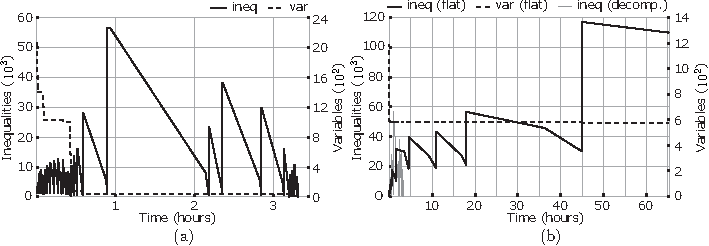
\includegraphics{figures/newDecompFig2.pdf}
	\caption{Size progression for the 8-section model (a) with decomposition and (b) flat.}
	\label{fig:8parts}
\end{figure} \\
\indent When considering each subsystem in a decomposition as a system in itself, in general, the number of inequalities after each call to \Call{FME-SingleVar}{} in Algorithm~\ref{alg:FMEF} grows to begin with, as does the number of inequalities before this call. This continues until there are a few variables left, where both these numbers decrease. For the decomposed algorithm, though the number of inequalities grow after each FME-step, most of them are redundant or almost redundant. The same does not hold for the flat projection of the complex VSMs (at least not for the steps that are completed within the time limit). On the contrary, many of the produced inequalities are non-redundant, increasing the likelyhood that even more inequalities will be produced in the next elimination and that the redundancy removal will take longer time. We also note that the runtime, even for the decomposed projections, are not exactly small, and the main part of the execution time is spend doing redundancy removal. However, as mentioned in the introduction, these calculations only need to be done once per vessel class. \\
\indent As a use-case example, the VSMs and their projected VCMs have been optimized for revenue. Each transported container yields a fixed revenue based on its type.
%TODO needs at least some explanation
 Table~\ref{tab:usingProjections} shows the number of iterations (iter), the deterministic time in ticks (time) and the optimal objective value (obj) in 10M\$. It likewise shows how many times faster, the projections are w.r.t. iterations and deterministic time, as well as the difference in objective value in percentage. For comparison, the number of iterations, deterministic time and objective value is shown for the simple VCM, too.
\begin{table}[tb]
\caption{Iterations, time and objective values for the VSMs and VCMs.}
\label{tab:usingProjections}
\centering
\btablesize
\begin{tabular}{l|r@{\:\;}r@{\:\;}r|r@{\:\;}r@{\:\:\:}r|rrr}
&\multicolumn{3}{c|}{VCM}&\multicolumn{3}{c|}{VSM}&\multicolumn{3}{c}{Difference}\\
					&iter&time  &obj 	 &iter  &time  &obj	&iter 			 &time					&obj\\ 
\hline
%No weights&	11 & 0.05 & 8.63 &	363 & 2.64 &8.08&$\times$33.0&$\:\times$52.8&$\:$6.8$\%$\\
No hydro. 	&  9 & 0.04 & 7.87 &	188 & 5.48 &6.22&$\times$20.9&$\:\times$137 &$\:$26.5$\%$\\
2 sections	& 14 & 0.29 & 6.09 &	251 & 5.88 &6.07&$\times$17.9&$\:\times$20.3&$\:$0.196$\%$\\
4 sections 	& 13 & 0.18 & 6.17 &  228 & 4.95 &6.16&$\times$17.5&$\:\times$27.5&$\:$0.153$\%$\\
6 sections 	&  9 & 0.20 & 6.17 &  227 & 5.02 &6.18&$\times$25.2&$\:\times$25.1&$\:$0.202$\%$\\
8 sections 	& 12 & 0.14 & 6.21 &  233 & 4.79 &6.18&$\times$9.4&$\:\times$34.2&$\:$0.490$\%$\\
\bottomrule
Simple VCM&  4 & 0.02 &10.7\phantom{0}\\
\end{tabular}
\etablesize
\end{table}
As can be seen from the numbers in Table~\ref{tab:usingProjections}, in general, VCMs are much faster to solve than their corresponding VSMs. More specifically there are approx. 17-21 %33
 times fewer iterations and 20-34 times fewer ticks for the complex models (137 for the non-complex one). %, which corresponds to a difference between 94\% and 97\% of the number of iterations, and 96\% and 99.5\% CPLEX ticks, respectively. 
Meanwhile the difference in objective value is only modest; for the complex model, the difference is at most 0.5 \%. %, while the other %two models have a difference of 6.8 and 26.5 \%, respectively. 
When comparing to the simple model, we see that this model of course is even faster, % (between 41-97 times (iterations) and 132-294 (ticks)), 
but the difference in objective is also between 72\% and 76\% for the last 5 models. Hence, our results confirm the experiments by Delgado \cite{AlbertosThesis} showing a substantial revenue overestimation of capacity models used in liner shipping today. \\

Beside the VSM, we have studied another block-angular structured system, namely one describing a multi-commodity flow problem.  
In short, this problem considers a graph on which a number of commodities can flow on the edges. Each edge has a capacity (upper bound) for each commodity as well as a common total capacity. Demands and supply are modelled as variables, and we want to examine the relationship between the supply and demand of the commodities without having to care about how the items flow in the internal nodes. This can be done by eliminating all other variables than the ones denoting the demands and supply of each commodity. We have generated the flow graph shown in Figure~\ref{fig:multiflow} with inspiration from the Chen.DSP collection \cite{JLFP93}. 
\begin{figure}[tb]
	\centering
		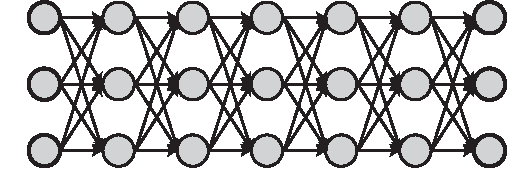
\includegraphics[scale=0.5]{figures/multiflow2.pdf}
	\caption{A ``layered''  graph for a multi-commodity flow problem.}
	\label{fig:multiflow}
\end{figure}
It consists of seven ``layers'' with three nodes each, and there are two commodities. The capacity for each commodity and edge is 0 with a probability of 5\% and otherwise drawn from a uniform distribution between 5 and 15, while the common capacity of the edge $e$ is 0 with probability 25\% and otherwise a number drawn from the uniform distribution between $s-1$0 and $s$, where $s$ is the sum of the individual capacities on $e$. A multi-commodity flow problem is naturally block-structured with a block for each commodity, but it contains usually many global constraints. Therefore, instead of using these blocks to decompose the system, we divide the graph into smaller subgraphs and use these as blocks. 
%TODO Ah, come on
Similarly to Table~\ref{tab:projections}, Table~\ref{tab:multicom} shows the size of the original model and the projections resulting from a flat and decomposed projection, respectively. Figure~\ref{fig:multicom} shows the progression over time of the number of inequalities and number of variables left to be projected, for both the flat and decomposed projection algorithm.
\begin{table}[tb]
\caption{Size of projection of a multi-commodity flow model.}
\label{tab:multicom}
\centering
\btablesize
\begin{tabular}{l|r@{ / }r@{ / }r@{ / }r|r}
&\multicolumn{4}{c|}{Size}&\multicolumn{1}{c}{Time}\\
											&ineq (eq)&var &nzs &dens&\\
\hline
Original							&204 (42) & 120& 444&2.17&\multicolumn{1}{c}{-}\\
Presolved							& 59		  &  79& 201&3.41&\multicolumn{1}{c}{-}\\
Projected, decomposed	& 17 (2)  &  12&  61&3.59& 2h \phantom{9}9m \\
Projected, flat				& 17 (2)  &  12&  53&3.12& 17h 41m\\
\end{tabular}
\etablesize
\end{table}
Also here we see a reduction in the number of inequalities, variables and non-zero entries, of 3.5, 6.6, and 3.3/3.8 times, respectively (in both cases) compared to the presolved model. The density stays almost the same; for the decomposed model, the density increases with 5.3 \%, while the density decreases with 8.5\% for the flat projection. This is not as large a reduction as for the VSMs, however, the unprojected models are also smaller to begin with. 
\begin{figure}[tb]
	\centering
		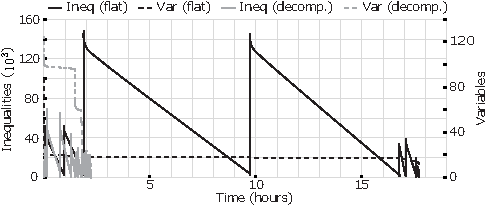
\includegraphics{figures/newMultiComGraph2.pdf}
	\caption{Size progression during projection of a multi-commodity flow problem.}
	\label{fig:multicom}
\end{figure}

%%%%%%%%%%%%%%%%%%%%%%%%%%%%%%%%%%%%%%%%%%%%%%%%%%%%%%%%%%%%%%%%%%%%%%%%%%%%%%%
\section{Related Work} \label{sec:relatedwork}
Other FME-based frameworks for projection includes \cite{simon05,lukatskii08,shapot12}. Similar to our framework, these use simplifications, redundancy removal and approximation-procedures. The latter uses the extreme-point method of \cite{huynh92}, while the boundary-approximation of \cite{lukatskii08,shapot12} involves a successive increase of the allowable deviation from the feasible area and a permissible maximal ratio of removed non-redundant inequalities. Seen from the perspective of capacity models, both frameworks are used on quite small systems. Furthermore, the systems in \cite{simon05} are also sparse. Our FME-based framework is to our knowledge the first that can take advantage of block-angular structure in the system. 

Other methods exist for computing the projection of a feasible area of a constraint system, that are not based on FME. The method in \cite{huynh92} finds extreme points in the projection space incrementally. It can therefore also be used to approximate the projection as is done in \cite{simon05}. It is recommended for dense systems. Another example is the method introduced in \cite{jones04}, which computes all facets of the projection iteratively using a face-lattice. This method is recommended by the authors for polytopes with a low facet count and a high vertex count.

%%%%%%%%%%%%%%%%%%%%%%%%%%%%%%%%%%%%%%%%%%%%%%%%%%%%%%%%%%%%%%%%%%%%%%%%%%%%%
\section{Conclusion}\label{sec:conclusion}
This paper has introduced a novel FME projection framework that automatically translates a linear stowage model (VSM) into a smaller sized capacity model (VCM) by projecting unneeded variables. To our knowledge, our framework is the first to exploit a block-angular structure for projection and apply massive parallelization of computations. Our results show that the projected VCMs are reduced by an order of magnitude both in number of inequalities and number of non-zero entries. The VCMs including hydrostatic constraints are solved 20-35 times faster than their corresponding VSMs. Similar results are achieved for at multi-commodity flow problem. Future work includes further parallelization and approaches to automatically estimate the best way of decomposing a given system as well as testing the framework on further block-angular problems.

\subsection*{Acknowledgements}
%\small 
We would like to thank Stefan R{\o}pke, Thomas Stidsen, and David Pisinger for discussions on applications of the FME framework beyond container vessel capacity models. This research is supported by the Danish Maritime Fund, Grant No. 2016-064.

\bibliographystyle{abbrv}
\bibliography{bibfile}
\end{document}
